\chapter{Turbostratic carbons II: Impregnation methods}
\label{ch:impregnation}

\newpage

\section{Introduction}

\section{Synthesis}
The author investigated additional precursors with high amounts of cellulosic material, therein using small amounts of porogen, and mixing the precursor and porogen in such a manner as to both minimise the distance between porogen and precursor, and evenly distribute the porogen. Firstly, sawdust-derived carbons were made by incorporating KOH at weight ratios between 0.00 and 2.00 into the hydrothermal carbonisation step, drying the resultant slurry overnight at $\rm 100\  ^{\circ}C$ and then activating at $\rm 800\ ^{\circ}C$ as usual. Hydrothermal carbonisation occured at 200, 250 or 300 $\rm ^{\circ}C$. These sawdust-derived hydrochars are designated \textit{SAx.xx-HHH} where the prefix \textit{SA} indicates activated sawdust, \textit{x.xx} is the KOH:sawdust ratio and \textit{HHH} is the hydrothermal carbonisation temperature. All samples were washed in the normal manner following activation. The hydrothermally carbonised intermediates are referred to as \textit{SHx.xx-HHH} to differentiate from the activated samples.
% should the lower TTT samples be included?

Additionally, sodium carboxymethyl cellulose (see figure \ref{fig:nc_structure}) was used as a precursor for direct (without hydrothermal carbonisation) activation. The porogen in this case is the sodium carboxymethyl group, and the porogen:precursor ratio is controlled by the degree of substitution. Samples are designated as \textit{NCx.x-TTT} where \textit{NC} indicates sodium carboxymethyl cellulose, \textit{x.x} is the degree of substitution, and \textit{TTT} is the activation temperature. Values for \textit{x.x} were 0.0, 0.7, 0.9, and 1.2 and \textit{TTT} was 600, 700, or 800 $\rm ^{\circ}C$.

\begin{figure}[h]
    \centering
    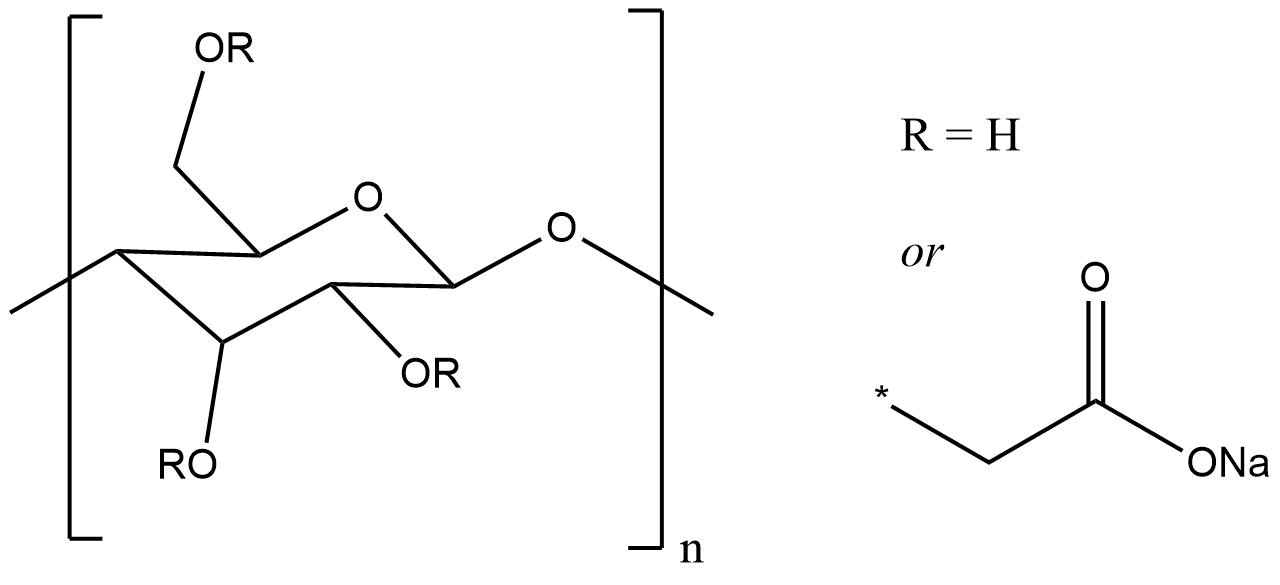
\includegraphics[width=0.8\columnwidth]{4-syntheses/figs/nc_structure.png}
    \caption{Structure of sodium carboxymethyl cellulose. Degree of substitution (DS) is taken as the average number of sodium carboxymethyl groups (\ce{-CH2COONa}) per monomer.}
    \label{fig:nc_structure}
\end{figure}

\section{Results \& Discussion}

\section{Conclusion}

\bibliographystyle{rsc}
\bibliography{bibliography/bib}

\section*{Appendix}